\documentclass[nofootinbib,prd,superscriptaddress,twocolumn]{revtex4}
\usepackage{amsmath,graphicx,hyperref}
\usepackage{slashed}
\usepackage{epstopdf}
\usepackage{color}
\usepackage[dvipsnames]{xcolor}


%%%%%%%%%%%%%%%%%%%%%%%%%%%%%%%%%%%%%%%%%%%%%%%%%%%%%%%%%%%%%%%%%%%%%%
%%%%%%%%%%%%%%%%%%%%%%%%%%%%% Command %%%%%%%%%%%%%%%%%%%%%%%%%%%%%%%%
%%%%%%%%%%%%%%%%%%%%%%%%%%%%%%%%%%%%%%%%%%%%%%%%%%%%%%%%%%%%%%%%%%%%%%

\newcommand{\fms}[1]{{#1}\!\!\!/}
\newcommand{\fmsl}[1]{{#1}\!\!\!\!/}

\newcommand{\mc}{\mathcal}
\newcommand{\mr}{\mathrm}
\newcommand{\mP}{\mathcal{P}}
\newcommand{\mO}{\mathcal{O}}

\newcommand{\be}{\begin{equation}} 
\newcommand{\ee}{\end{equation}} 
\newcommand{\beq}{\begin{equation}} 
\newcommand{\eeq}{\end{equation}} 
\newcommand{\bea}{\begin{eqnarray}} 
\newcommand{\eea}{\end{eqnarray}} 

\newcommand{\ov}{\overline}
\newcommand{\pp}{\perp}
\newcommand{\dg}{\dagger}
\newcommand{\n}{\overline{n}}
\newcommand{\nn}{\frac{\fms{\overline{n}}}{2}} 
\newcommand{\nnn}{\frac{\fms{n}}{2}} 

\newcommand{\bl}[1]{{\bf{#1}}}
\newcommand{\bla}[1]{|{\bf{#1}}|}
\newcommand{\blp}[1]{{\bf{#1}}_{\perp}}
\newcommand{\blpu}[1]{{\bf{#1}}^{\perp}}
\newcommand{\blpa}[1]{|{\bf{#1}}_{\perp}|}
\newcommand{\bs}[1]{\boldsymbol{#1}}
\newcommand{\bsp}[1]{{\boldsymbol{#1}}_{\perp}}

\newcommand{\ds}{\displaystyle} 
\newcommand{\nnb}{\nonumber} 

\newcommand{\as}{\alpha_s} 

\newcommand{\eps}{\epsilon} 
\newcommand{\veps}{\varepsilon} 

\newcommand{\UV}{\veps_{\mr{UV}}}
\newcommand{\IR}{\veps_{\mr{IR}}}

\newcommand{\La}{\Lambda^2_{\rm{alg}}}

%--- journals
\newcommand{\physrep}{Phys. Reports}
\newcommand{\mnras}{Mon. Not. R. Astron. Soc.}
\newcommand{\apjl}{Astrophys. J. Lett.}
\newcommand{\jcap}{J. Cosmol. Astropart. Phys.}

%--- for comments
\newcommand{\arz}[1]{{{\bf{\color{BrickRed}[ARZ: #1]}}}}

%%%%%%%%%%%%%%%%%%%%%%%%%%%%%%%%%%%%%%%%%%%%%%%%%%%%%%%%%%%%%%%%%%%%%%

\bibliographystyle{apsrev}

%\topmargin 0.0 in

\begin{document}

\baselineskip 3.0ex 

\vspace*{18pt}

%%%%%%%%%%%%%%%%%%%%%%%%%%%%%%%%%%%%%%%%%%%%%%%%%%%%%%%%%%%%%%%%%%%%%%
%%%%%%%%%%%%%%%%%%%%%%%%%%%%% Title %%%%%%%%%%%%%%%%%%%%%%%%%%%%%%%%%%
%%%%%%%%%%%%%%%%%%%%%%%%%%%%%%%%%%%%%%%%%%%%%%%%%%%%%%%%%%%%%%%%%%%%%%

\title{Updated Constraints on Self-Interacting Dark Matter from Supernova 1987A}

\def\Pitt{Pittsburgh Particle Physics Astrophysics and Cosmology Center (PITT PACC) \\ Department of Physics and Astronomy, University of Pittsburgh, Pittsburgh, Pennsylvania 15260, USA}

\author{Cameron Mahoney}
\email[E-mail:]{cbm34@pitt.edu}
\affiliation{\Pitt}
\author{Adam K. Leibovich}
\email[E-mail:]{akl2@pitt.edu}
\affiliation{\Pitt}
\author{Andrew R. Zentner}
\email[E-mail:]{zentner@pitt.edu}
\affiliation{\Pitt}  

\begin{abstract} 
\baselineskip 3.0ex   
Abstract?
\end{abstract}

\maketitle 

%%%%%%%%%%%%%%%%%%%%%%%%%%%%%%%%%%%%%%%%%%%%%%%%%%%%%%%%%%%%%%%%%%%%%%

%------------------------- Introduction ---
\section{Introduction}

A nearly overwhelming preponderance of observational evidence indicates that a form of nonrelativistic, nonbaryonic, 
dark matter constitutes the vast majority of mass in the Universe and drives the formation of cosmic structure. 
The pace of the quest to identify the dark matter is accelerating on many fronts. Weakly-interacting massive 
particles (WIMPs) have received the most attention as dark matter candidates (see Ref.~\cite{jungman_etal96} for a review). 
Dark matter particles that interact with standard model particles only weakly, while interacting among themselves 
much more strongly have been studied as an alternative to WIMP scenarios in many contexts 
\cite{carlson_etal92,deLaix_etal95,atrio-barandela_davidson97,spergel_steinhardt00,hogan_dalcanton00,mohapatra_teplitz00,
dave_etal01,hisano_etal04,hisano_etal05,pospelov_etal08,arkani-hamed_etal08a,lattanzi_silk08,ackerman_etal09,feng_etal09,
kong_etal15} \arz{Need to add some more recent references here.} 
and constraints on self-interacting dark matter (SIDM) models have been explored by many authors \cite{yoshida_etal00,gnedin_ostriker01,miralda-escude02,randall_etal08,kamionkowski_profumo08,zentner09,robertson_zentner09,pieri_etal09,spolyar_etal09,finkbeiner_etal09,
slatyer_etal09,bramante_etal14,albuquerque_etal14,kaplinghat_etal14,chen_etal14,feng_etal16,catena_widmark16}.
In this paper, we revisit and update astrophysical constraints on SIDM models from 
supernova cooling, finding constraints that are considerably less restrictive than in 
previous work. 
\arz{Might want to add a comment about SIDM affecting small-scale structure in CDM, the satellites problems and core/cusp problems.}


SIDM models in which large self-interaction cross sections are mediated by sufficiently light 
bosons ($M \lesssim 100$~GeV) can be constrained astrophysically using supernovae, particularly 
SN1987A. Light gauge bosons will be produced within the hot supernovae core and 
radiated from the supernova. This non-standard energy loss mechanism can result in an energy loss rate 
from the supernova core that is inconsistent with observations of SN1987A, analogous to the 
classic constraint on axions \cite{raffelt96_book}. This mechanism was already exploited by 
\cite{dent_etal12} (and \cite{rrapaj_reddy16}, with a slight modification) (\arz{Cameron, add others of which you may be aware.}) 
to constraint dark electromagnetism models of SIDM in which the self-interaction arises from a Yukawa potential and the 
vector boson is kinetically mixed with the standard model photon.


As we mentioned above, we find SN1987A constraints on dark photon SIDM models that are considerably different 
from those of \cite{dent_etal12}. If correct, this has important consequences. The Snowmass white paper by Kaplinghat, 
Tulin, and Yu \cite{kaplinghat_etal13_whitepaper} nicely summarizes a variety of constraints on dark electromagnetism models of 
SIDM. One point that is clear from Ref.~\cite{kaplinghat_etal13_whitepaper} is that there is only a narrow range of 
viable photon mixing parameters that can lead to production of SIDM in the early universe, while evading all constraints, 
including the constraint of \cite{dent_etal12}. Our results suggest that the SN1987A constraints from Ref.~\cite{dent_etal12} 
are too restrictive. The less restrictive constraints that we quote open up a space of unrestricted mixing parameters that 
ranges over two orders of magnitude. Interestingly, the parameter space opened by our updated constraints corresponds to a 
space that may a significant impact on cosmological structure formation, particularly the structures of dark matter halos and galaxies. 


The discrepancy between our result and that of Ref.~\cite{dent_etal12} is due to several factors. First, it is straightforward to 
demonstrate that the kinematical relationships in given in Appendix A of Ref.~\cite{dent_etal12} are incorrect. Second, the 
squared matrix elements given in Eq.~(A3) and Eq.~(C18) of Ref.~\cite{dent_etal12} are incorrect. Our squared matrix elements 
are considerably more complicated. There appear to be a number of errors that led to the incorrect squared matrix elements in 
Ref.~\cite{dent_etal12}. At the very least, these errors include simplification using the incorrect kinematics and neglect of the 
mass of the gauge boson (which, while legitimate for the $\sim$meV-mass axion, is not justified in this context). Additional 
discrepancies must be present, the causes of which are not apparent from the exposition, 
because the squared matrix elements in Eq.~(A3) and Eq.~(C18) of Ref.~\cite{dent_etal12} 
do not obey the correct symmetries under interchange of the incoming or outgoing baryon momenta. 
Given these errors, we suggest that our results should supercede these previously-published constraints.

The remainder of this paper is organized as follows. In Section~\ref{section:model}, we discuss 
dark photon models. We describe our calculation of SN1987A constraints on SIDM in 
Section~\ref{section:computational} and present our primary results in Section~\ref{section:results}. 
We summarize our work and draw conclusions in Section~\ref{section:conclusions}. 

%---- Model Details
\section{Dark Photon Model of SIDM}
\label{section:model}

We consider constraints on SIDM specifically within the context of dark electromagnetism models. 
Dark electromagnetism models are models in which a hidden, dark, sector contains a broken U(1)$'$ 
symmetry and the U(1)$'$ gauge boson is kinetically mixed with the standard model photon. For the 
purposes of this study, this is important because it demands that the Lagrangian contains terms such as 
%
\begin{equation}
\mathcal{L}_{\mathrm{int}} = g_{\chi} \bar{\chi} \, \tilde{\slashed{A'} } \chi + q \bar{f}\, \tilde{\slashed{A} } f, 
\end{equation}
%
where $\chi$ is the dark matter, $g_{\chi}$ is the dark coupling, $\tilde{A}'$ is the dark gauge boson, 
$f$ is a standard model fermion of charge $q$, and $\tilde{A}$ is the standard model gauge boson. 
The kinetic mixing causes the $\tilde{A}$ to be an admixture of the massless photon, $A$, and 
the dark photon, $A'$ of mass $m_{\mathrm{A'}}$, so that the dark matter particles are coupled to the standard model 
fermions with a coupling constant $\epsilon q$, where $\epsilon$ is the kinetic mixing parameter. 
The first term in this interaction gives rise to the dark matter self-interactions. 

Dark gauge bosons are produced in astrophysical environments such as supernova 
cores via brehmsstrahlung off of standard model particles. This brehmsstrahlung 
occurs through the $\epsilon q$ coupling. The rate of brehmsstrahlung 
also depends upon the mass of the $A'$. Consequently, 
supernova cooling can constrain the mixing $\epsilon$ as a function of 
$m_{A'}$ for such models and producing such a constraint is the 
primary aim of this paper.


%----- Computational Details
\section{Computational details}
\label{section:computational}
	
	The process we are considering, the bremsstrahlung of a dark photon from nucleon-nucleon scattering, is similar in many ways to the classic calculation of axion emission from supernova cooling. The differences arise due to the mass of the dark photon, which can be on the order of the temperature of the supernova.  This leads to different kinematics compared to the axion case.  However, the calculation roughly follows the analogous calculation for axions, as laid out by Raffelt, which we briefly review below.  As in the classical axion calculation, we will use the one-pion exchange (OPE) approximation.  
	
\subsection{Bremsstrahlung amplitude calculation}
	 There are two processes to consider: the $pp$ scattering with the bremsstrahlung of the dark photon off the proton, $ p+p \rightarrow p+p+A$, and the $pn$ scattering with bremsstrahlung off the proton or the charged pion, $ p+n \rightarrow p+n+A\ $. For the $pp$ case there are eight tree-level diagrams, with the emission of the $A'$ from each of the external legs, as shown in Fig. , while for the $pn$ case there are five diagrams, including when the $A'$ is emitted from the exchanged pion, as shown in Fig. .
	
The calculation of these diagrams is straightforward, and is described in the appendix. Having obtained the diagrams the calculation diverges from the axion bremsstrahlung calculation, since in the kinematic region of interest for supernova explosions the mass of the $A'$ boson is not necessarily negligible. The kinematic relations are thus \bea 
p_1 \cdot p_2 &=& M_N^2 - \frac{l^2}{2} - \frac{k^2}{2} + p_2 \cdot q_a,\\
p_1 \cdot p_3 &=& M_N^2 + k \cdot l - \frac{k^2}{2} + p_3 \cdot q_a,\\  
p_1 \cdot p_4 &=& k \cdot l + M_N^2 - \frac{l^2}{2} + p_4 \cdot q_a, \\
p_2 \cdot p_3 &=& M_N^2 - \frac{l^2}{2}, \\ 
p_2 \cdot p_4 &=& M_N^2 - \frac{k^2}{2},\\
p_3 \cdot p_4 &=& k \cdot l + M_N^2 - \frac{l^2 + k^2}{2}.
\eea
Unfortunately, with these relations it does not seem to be possible to simplify the amplitude into an analytically usable form without making unjustified approximations, and so the final expression for the spin-averaged squared matrix element, $ \mathcal{M}^2_{pp}$, contains some two hundred and fifty terms, and thus we do not reproduce that result here. The pn calculation likewise results in a very large and unwieldy expression for $ \mathcal{M}^2_{pn}$. \footnote{At this point we diverge from Ref.~\cite{dent_etal12} for two reasons.  One, they use the kinematics as if the $A'$ were massless, as in the axion calculation, and independent of that choice, their squared matrix element does not respect the correct exchange symmetry, as can be seen by inspection of their Eq. (A.3), with their claim that only the coefficient $C_k$ appearing in that equation is nonzero.}


\subsection{Streaming limit}
The first and simplest bound that may be obtained arises from assuming that all produced particles leave the supernova, carrying their energy with them. The constraint is derived simply by requiring that the energy loss through this cooling channel be roughly less than the cooling from neutrino emission; any greater, and it would have an observable effect on supernova cooling.

The actual quantity of interest therefore is the rate of energy emission through dark bosons. From the spin-summed squared amplitudes already found, this is obtained by integrating over the phase space, and adding a factor of energy of the emitted particle.
\beq
Q_i = \int (2\pi)^4 E_A \sum_{spins} \mathcal{M}^2_i f(p_1) f(p_2)\delta(p_1+p_2-p_3-p_4-q_a) d\Pi,
\eeq
where $d\Pi$ is the Lorentz-invariant phase space, $ E_A $ is the energy of the emitted boson, and $ f(p) $ are the initial occupation numbers. The nucleons in the core are comfortably non-degenerate and non-relativistic, so  the Pauli blocking factor is omitted and the Maxwell-Boltzmann distribution is used  
\beq
f(p) =  \frac{n_b}{2} (\frac{2 \pi}{M_N T})^{3/2} e^{-\frac{\textbf{p}^2} {2 M_N T}}.
\eeq
	
The integration is performed numerically to obtain $ Q_i$, which is the rate of energy emission per unit volume associated with either the $pn$ or $pp$ process. To obtain the dark gauge boson luminosity, it is assumed that production takes place in a core volume $V$ of radius 1 km, giving $ \mathcal{L}_A = V(Q_{pp} + Q_{pn}) $. The luminosity $\mathcal{L}_A $ is a complicated function of $ m_A $ and $ T $, but is simply proportional to the square of the parameter $ \epsilon $.  Pulling that out of the expression gives a constraint 
\beq
\epsilon^2 I_A(m_A, T) \le \mathcal{L}_\nu
\eeq
or a bound on the coupling of 
\beq 
\epsilon \le \sqrt{\frac{4.1 \times 10^{37} MeV^2}{I_A(m_A, T)}} 
\eeq 
and the exclusion region is generated by varying the mass. 

\subsection{Decay limit}
The constraint from the streaming limit above provides an upper bound on the allowed coupling (or lower bound on the excluded coupling) by considering the production on the $A'$. Naively it might be expected that this suffices, in that all higher couplings are excluded. However, in order to function as a cooling channel, enough of the produced dark gauge bosons must escape the supernova. As the coupling increases, so do processes that prevent the escape, and so the excluded region has an upper bound, above which the luminosity again drops below the neutrino luminosity. The first such limit may be found by considering decay of the dark bosons into Standard Model particles, and assuming that these SM particles are trapped in the supernova core and contribute nothing to the cooling. The dark boson has a typical lifetime of 
\beq
l = \frac{3 E_{A}}{N_{eff} m_A^2 \epsilon^2},
\eeq
and so the fraction escaping the supernova before decaying is given by 
\beq
e^{r_{decay}/l} = e^{r_{decay} N_{eff} m_A^2 \epsilon^2/(3 E_A)}.
\eeq
To take this into account, the above exponential factor is simply appended to the phase space integrand, and the calculation then proceeds as before. The limit is derived from the same equation, with the only complication being the fact that $ I_A $ is now a function of $ \epsilon $, in addition to $ m_A, T $. This makes the numerical calculation slightly more complicated, but otherwise changes nothing of importance, with now the constraint a transcendental equation,  
\beq
\epsilon \le \sqrt{\frac{4.1 \times 10^{37} MeV^2}{I_A(m_A, T, \epsilon)}}.
\eeq
	
	
\subsection{Trapping limit}
The second constraint that produces an upper bound on the excluded region comes from considering trapping of dark bosons within the supernova. With a large enough coupling, the new particles will thermalize and then will be emitted from a spherical shell.  In this case the luminosity is given simply by the Steffan-Boltzmann law
\beq
\mathcal{L}_t  = 4\pi r^2 T_A^4 \sigma,
\eeq
where $ r $ is now the radius of the emitting shell and $ T_A $ its temperature. We can estimate $ r = 10$ km, since the density of the supernova drops drastically around that point. After taking that value for r, the bound on the luminosity translates into a bound on $ T_A $ 
\beq
T_A \le 9.586\rm\ MeV.
\eeq
That bound can then be translated into the desired bound on the coupling as a function of mass by assuming that the particles are emitted from an optical depth $ \tau = 2/3 $, and finding the temperature that corresponds to that optical depth. This is a somewhat involved calculation.
First, one needs a model for the density and temperature in the supernova. Following \cite{dent_etal12}, we assume 
\bea
\rho &=& \rho_p \left(\frac{R}{r}\right)^n,\\
T &=& T_R \left(\frac{\rho(r)}{\rho_R}\right)^{1/3},
\eea
with $  \rho_p  = 3\times10^{14}\ {\rm g/cm}^3, T_R = 30$ MeV, and taking $ n = 5 $. The optical depth is given by 
\beq
\tau = \int_{r_x}^{\infty} \kappa \rho dr,
\eeq
where $ \kappa$ is the opacity.  To find the opacity, we start from the reduced mean Rosseland opacity 
\beq
\frac{1}{\kappa \rho} = \int_{m_x}^{\infty} \frac{15}{4 \pi^4 T^5} \frac{E_A^2 e^{E_A/T} \sqrt{E_A^2 - m_A^2}}{(e^{E_A/T}-1)^2} l_A dE_A,
\eeq
where $ l_A $ is the mean free path. 
	
The inverse mean free path can readily be obtained by modifying $ Q_i $, the expression for the energy loss rate, as follows: removing the factor of $ E_A $ and the phase space integral over $ q_A $, and adding a factor of $ e^{E_A/T} $ for detailed balance. This gives the inverse mean free path as a function of mass and coupling. Again the required integration is performed numerically. This then allows the calculation of $ \kappa_x $. The inverse opacities for the $pn$ and $pp$ processes add, giving the total opacity $ \kappa^{-1} = \kappa_{pp}^{-1} + \kappa_{pn}^{-1} $
	
Having obtained an expression for $ \kappa $, we can now find the optical depth as follows: define a new quantity $ \tau_R = \kappa_R \rho_R R $. We then have 
\beq \kappa \rho R = \tau_R (\frac{\rho}{\rho_R})^2 (\frac{T_R}{T})^{3/2}  \eeq
This is combined with the expressions for the density and temperature as a function of r and plugged in to the integral expression for the optical depth to obtain 
\bea \tau_x &=& \int_{r_x}^{\infty} \tau_R (\frac{R}{r})^{3n/2} \\
 &=& \frac{\tau_r}{\frac{3n}{2}-1} (\frac{T_A}{T_R})^{(9/2-3/n)} \eea
and the bound on the coupling is finally found by requiring  $ \tau_x(\epsilon,m_A) \le 2/3 $
	
	
	
\subsection{Phase Space Integration}
In every case calculating the bound requires integrating an expression involving the long and complicated Bremsstrahlung amplitude, which unfortunately could not be done analytically without making unjustified approximations. The integration was consequently performed numerically using the Monte Carlo routines provided by the Cuba library. Employing kinematic relations did not seem to reduce the complexity of the problem, so in the interests of reducing the number of possible mistakes the kinematics were done by brute force. We integrated over the entire phase space explicitly in terms of the eleven variables of $ \vec{p_1}, \vec{p_2}, \vec{p_3}, \hat{q_a} $, then fixed $ p_4 $ using the 3-momentum part of the delta-function and used an unpleasantly complicated equation obtained from the energy delta-function to fix the remaining one free momentum amplitude - in our case we chose this to be $ q_a $, the momentum of the emitted boson. At each step points resulting in unphysical configurations were discarded, and the remaining points were then plugged in to the appropriate amplitude, and then that result used as the integrand. The numerical integration routine used was the \textit{Suave} method provided by CUBA, which combines importance sampling and adaptive subdivision; this method seemed to provide the best compromise between computation time and error. 
	
Once the integration is complete the calculation of the trapping and streaming limits is a straightforward application of the equations previously derived, and proceeded as outlined above. The decay limit is somewhat harder, since $ \epsilon $ appears on both sides of the equation. Again we employed an unsubtle approach to solving the problem: $ \epsilon $ was set to an arbitrary value where the constraint was satisfied, and then iteratively reduced until the constraint was no longer satisfied. This obviously introduces another source of error, but with a sufficiently small interval in $ \epsilon $ this is negligible. The one further slight complication is that at after a certain value of $ M_A $ the decay limit rapidly goes to zero, at which point the procedure was terminated.
	
We then scanned over the desired range of values for $ M_A $ and output the three limits - trapping, decay, and streaming - at each point. The complexity of the integration was such that errors remained relatively large even with highest practicable number of samples.

The calculation is dependent on a number of constants. We chose the following values as roughly typical of supernovae: T, the temperature of the supernova core, was set to 30 MeV; r, the radius of the supernova core, to 1 km; $ R $, the distance at which decay products are trapped, to 10 km; $ \mathcal{L} $, the luminosity bound, to $ 10^{53} erg/s $; and $ \n_b $, the baryon number density in the supernova interior, to $ 1.79*10^{38} cm^{-3} $. 


%-------------------- RESULTS
\section{Results}
\label{section:results}

\begin{figure}[th]
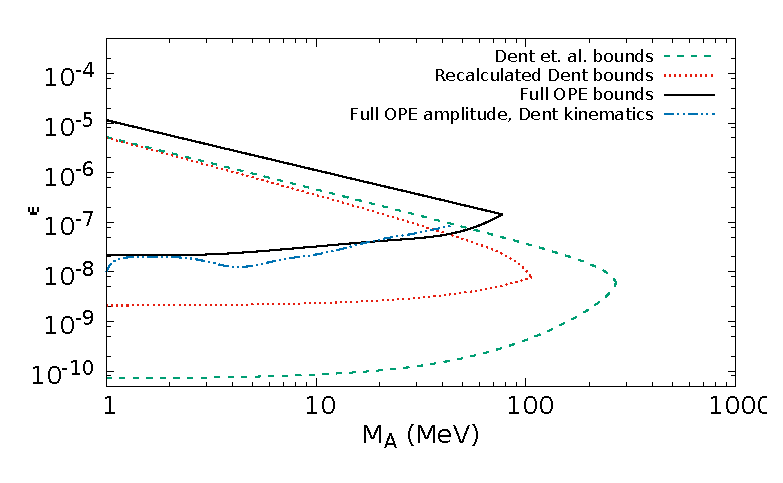
\includegraphics[width=9cm]{stages.eps}
\caption{The changes in the bounds generated as each stage of the calculation departs from Ref.~\cite{dent_etal12}. Interestingly the kinematics have apparently relatively little effect.
\arz{Cameron, several to-do items for this figure. On the y-axis, the symbol should be "$\epsilon$" rather than 
"e". Can we write numbers as "$10^{-9}$" rather than "1e-09" and so on? Can we make the axis labels and 
tick mark labels larger? Can you make all of the lines thicker? Can you make each of the four lines a distinct color?}
}
\end{figure}

Let's put some text here.

\begin{figure}[th]
	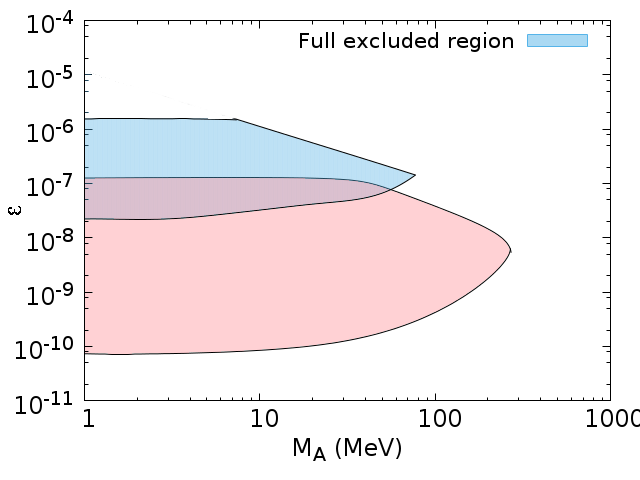
\includegraphics[width=9cm]{endtoend.png}
	\caption{A comparison of the final result for the excluded region with the result from Ref.~\cite{dent_etal12}. The excluded region is clearly significantly less restrictive, and opens up the region of parameter space for $\epsilon \approx  1e-8-9 $.
\arz{Cameron, some similar comments as for Figure 1. Can we write numbers as "$10^{-9}$" rather 
than "1e-09" and so on? Can we make the axis labels and tick mark labels larger?}	
	}
\end{figure}


%--------------------------- CONCLUSIONS
\section{Discussion and Conclusions}
\label{section:conclusions}


	The revised approach produce constraints that are significantly weaker than the previous work, and that largely reproduce constraints already obtained from beam dump experiments. 



%------------ APPENDIX
\appendix
\section{Bremsstrahlung diagrams}
	Each of the $p-p-\pi $ vertices contribute a factor of $g_{pp}$,  the pseudoscalar pion-nucleon coupling. $f_{pp}$, the pseudovector pion-nucleon coupling, is related by $g_{pp} = \frac{2M_N}{m_\pi} f_{pp} $. The $ p-p-A' $ vertex contributes $e\epsilon \gamma_\mu$, where $\epsilon$ is the mixing strength between the photon and dark photon. Labeling the contributions according to the Feynman diagrams in Fig. , the matrix elements are 
	\bea
	M_1 &=& \frac{4 M_N}{ m_\pi} \frac{f_{pp}^2 e \epsilon}{l^2-m_\pi^2
	}  \frac{1}{m_{A^\prime}^2 - 2 q_a \cdot p_1} \bar{u}(p_3) \gamma_5 u(p_2) \bar{u}(p4) \gamma_5 (\slashed{p}_1 - q_a +M_N)\slashed{\varepsilon} u(p_1),\\
	M_2 &=& \frac{4 M_N}{ m_\pi} \frac{f_{pp}^2 e \epsilon}{k^2-m_\pi^2
	}  \frac{1}{m_{A^\prime}^2 - 2 q_a \cdot p_1} \bar{u}(p_4) \gamma_5 u(p_2) \bar{u}(p3) \gamma_5 (\slashed{p}_1 - q_a +M_N)\slashed \varepsilon  u(p_1), \\
	M_3 &=& \frac{4 M_N}{ m_\pi} \frac{f_{pp}^2 e \epsilon}{l^2-m_\pi^2
	}  \frac{1}{m_{A^\prime}^2 - 2 q_a \cdot p_2} \bar{u}(p_3) \gamma_5 u(p_1) \bar{u}(p4) \gamma_5 (\slashed{p}_2 - q_a +M_N)\slashed \varepsilon  u(p_2), \\
	M_4 &=& \frac{4 M_N}{ m_\pi} \frac{f_{pp}^2 e \epsilon}{k^2-m_\pi^2
	}  \frac{1}{m_{A^\prime}^2 - 2 q_a \cdot p_2} \bar{u}(p_4) \gamma_5 u(p_1) \bar{u}(p3) \gamma_5 (\slashed{p}_2 - q_a +M_N)\slashed \varepsilon  u(p_2), \\
	M_5 &=& \frac{4 M_N}{ m_\pi} \frac{f_{pp}^2 e \epsilon}{l^2-m_\pi^2
	}  \frac{1}{m_{A^\prime}^2 + 2 q_a \cdot p_3} \bar{u}(p_4) \gamma_5 u(p_1) \bar{u}(p3) \slashed{\varepsilon} (\slashed{p}_3 + q_a +M_N)\gamma_5 u(p_2),\\
	M_6 &=& \frac{4 M_N}{ m_\pi} \frac{f_{pp}^2 e \epsilon}{k^2-m_\pi^2
	}  \frac{1}{m_{A^\prime}^2 + 2 q_a \cdot p_3} \bar{u}(p_3) \gamma_5 u(p_1) \bar{u}(p4) \slashed{\varepsilon} (\slashed{p}_3 + q_a +M_N)\gamma_5 u(p_2),\\
	M_7 &=& \frac{4 M_N}{ m_\pi} \frac{f_{pp}^2 e \epsilon}{l^2-m_\pi^2
	}  \frac{1}{m_{A^\prime}^2 + 2 q_a \cdot p_4} \bar{u}(p_3) \gamma_5 u(p_2) \bar{u}(p4) \slashed{\varepsilon} (\slashed{p}_4 + q_a +M_N)\gamma_5 u(p_1),\\
	M_8 &=& \frac{4 M_N}{ m_\pi} \frac{f_{pp}^2 e \epsilon}{k^2-m_\pi^2
	}  \frac{1}{m_{A^\prime}^2 + 2 q_a \cdot p_4} \bar{u}(p_4) \gamma_5 u(p_2) \bar{u}(p_3) \slashed{\varepsilon} (\slashed{p}_4 + q_a +M_N)\gamma_5 u(p_1),
	\eea
	where the exchange momenta are defined by $ k = p_2-p_4 $ and $ l = p_2-p_3 $, and the dark photon's polarization is given by $\varepsilon$. 
	For $pn$ scattering, four of the diagrams are simply the same as those given above. The only new Feynman diagram comes from bremsstrahlung off the internal pion, and results in  
	 \beq
	 M'_5 = \frac{4 M_N}{ m_\pi} \frac{f_{pn}^2 e \epsilon}{l^2-m_\pi^2
	 }  \frac{1}{(l-q_a)^2 - m_\pi^2} \bar{u}(p_4) \gamma_5 u(p_1) \bar{u}(p_3) u(p_2) (q_a - 2l)\cdot \varepsilon
	 \eeq
	 Note that these matrix elements agree with Ref.~\cite{dent_etal12}.
\acknowledgments

AKL was supported in part by NSF grant PHY-1519175.


\bibliography{draft}

\end{document}

%%%%%%%%%%%%%%%%%%%%%%%%%%%%%%%%%%%%%%%%%%%%%%%%%%%%%%%%%%%%%%%%%%%%%%
%%%%%%%%%%%%%%%%%%%%%%%%%%%%% Bibliography %%%%%%%%%%%%%%%%%%%%%%%%%%%
%%%%%%%%%%%%%%%%%%%%%%%%%%%%%%%%%%%%%%%%%%%%%%%%%%%%%%%%%%%%%%%%%%%%%%


%%%%%%%%%%%%%%%%%%%%%%%%%%%%%%%%%%%%%%%%%%%%%%%%%%%%%%%%%%%%%%%%%%%%%%

\end{document}